%%%%%%%%%%%%%%%%%%%%%%%%%%%%%%%%%%%%%%%%%%%%%%%%%%%%%%%%%%%%%%%%%%%%%%%%
\chapter{Android}
\label{sec:android}
%%%%%%%%%%%%%%%%%%%%%%%%%%%%%%%%%%%%%%%%%%%%%%%%%%%%%%%%%%%%%%%%%%%%%%%%

%=======================================================================
\section{Überblick}
%=======================================================================
Android ist ein Betriebssystems, welches primär für Smartphones und Tablets konzeptioniert ist. Das Betriebssystem basiert auf einen Linux Kernel und wird von der Open Handset Alliance (gegründert von Google) entwickelt \cite{overviewAndroid:singh}. Android ist eine freie Software, und das am schnellsten wachsende mobile Betriebssystem. Der Marktanteil von Android liegt seit 2014 bei über 80\% und sollte sich auch in den darauffolgenden Jahren bei dieser Prozentzahl halten, wie in der Abbildung \ref{figure:marketshare} zu sehen ist. \\
 
\begin{minipage}{\textwidth} 
	\centering	
	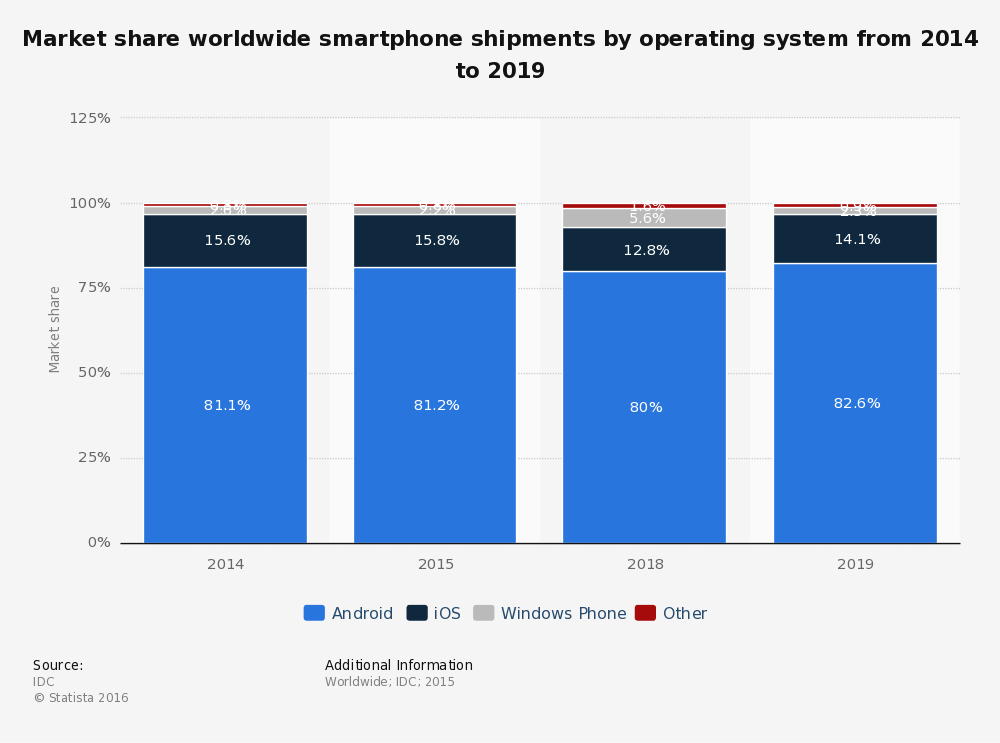
\includegraphics[width=0.65\textwidth]{figures/smartphone-os-market-share.png}
	\captionof{figure}{Marktanteil von mobilen Betriebssystemen \cite{statsticMobileOS}}
	\label{figure:marketshare}
	\vspace{2ex}
\end{minipage}

Durch die quelloffene Struktur des Betriebssystems ist Android bei vielen Konsumenten und Entwicklern sehr beliebt, wodurch viele Unternehmen ihre mobilen Applikationen auf dieses Betriebssystem ausrichten. Gemäß einer Vorhersage von IDC, wird Android zwar eine gewisse Prozentzahl an das Windows Phone Betriebssystem verlieren, aber weiterhin der Marktführer bleiben \cite{statsticMobileOS}. Aufgrund dessen wurde die Evaluierung der REST Frameworks auf Android ausgerichtet, um auch in den folgenden Jahren einen hohen Nutzerkreis erreichen zu können.

%=======================================================================
\section{Architektur}
%=======================================================================
Das Android Betriebssystem ist ein Stack von Software Komponenten, welche typischerweise in vier Bereiche gegliedert werden (vgl. \ref{figure:androidArchitekture}). Diese Bereiche sind der Linux Kernel, die Native Bibliotheken, die Laufzeitumgebung, das Application-Framework, und die Applikationen selbst \cite{androidTutorialOS}. \\

\begin{minipage}{\textwidth} 
	\centering	
	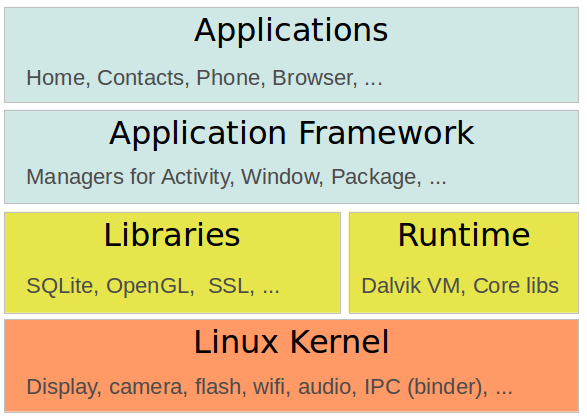
\includegraphics[width=0.65\textwidth]{figures/android_stack.png}
	\captionof{figure}{Android Architektur \cite{androidTutorialOS}}
	\label{figure:androidArchitekture}
	\vspace{2ex}
\end{minipage}

Beschreibung der Software Komponenten der Android Architektur \cite{overviewAndroid:singh}, \cite{androidTutorialOS}: 
\begin{itemize}
	\item \textbf{Applikationen}\\
	Die Applikationen stellen die oberste Schicht der Android Architektur dar. Einige Applikationen sind bereits auf jedem Smartphone vorinstalliert, wie beispielsweise ein SMS Client,  ein Browser, oder ein Kontaktmanager. Software Entwickler können ihre eigenen Applikationen schreiben und diese auf dem Smartphone installieren.\\
	Die zu entwickelnde App, sowie die zu evaluierenden REST-Frameworks befinden sich auf dieser Schicht - das REST-Framework und die Beispielimplementierung werden gemeinsam in eine .apk-Datei zusammengefasst.
	\item \textbf{Application-Framework}\\
    In der Application-Framework-Schicht befinden sich zahlreiche Java-Bibliotheken und Dienste, auf welche Software Entwickler bei der Applikationserstellung Zugriff haben. Wichtige Dienste sind dabei der Activity Manager, der Resource Manager, oder der Content Manager.
	\item \textbf{Native Bibliotheken}\\
	Die Nativen Bibliotheken stellen zahlreiche Funktionen für die Application-Framework-Schicht zur Verfügung, wie Grafik-Rendering, oder Web-Browsing. Alle diese Bibliotheken sind in C oder C++ geschrieben, und werden bei der Entwicklung von Applikationen durch Java Interfaces aufgerufen.
	\item \textbf{Runtime}\\
	Die Laufzeitumgebung besteht aus der Dalvik \acrfull{VM} und den Java Kernbibliotheken. Die Dalvik VM ist eine Java Virtual Machine, welche speziell für Android entwickelt und optimiert wurde.  Durch die  Dalvik VM kann jede Applikation in einem eigenen Prozess ausgeführt werden, in einer eigenen Instanz der Dalvik VM. \\
	Durch die Java Kernbibliotheken in der Laufzeitumgebung können Software Entwickler Android Applikationen mithilfe der Programmiersprache Java entwickeln.   
	\item \textbf{Linux Kernel}\\
	Der Linux Kernel stellt die unterste Schicht der Android Architektur dar, welcher leicht von Google abgeändert wurde. Der Kernel ist dabei die Schnittstelle zur Geräte Hardware (Kamera, Display etc.) und ist gleichzeitig für die Speicher- und Prozessverwaltung verantwortlich.
\end{itemize}
	
%=======================================================================
\section{Cross Compiling}
%=======================================================================	
Um eine Applikation auf Android ausführen zu können, muss eine .apk-Datei erstellt werden. Dazu wird als erstes eine .java-Datei vom Entwickler erstellt, welche den Quellcode der Applikation enthält. Danach wird mit einem Java-Compiler der Bytecode in Form von .class-Dateien erstellt. Dieser Bytecode wird mit dem dx-Tool aus dem Android SDK in eine .dex-Datei (Dalvik Executable) umgewandelt. Den Bytecode welche die Dalvik VM ausführt, ist daher kein Java-Bytecode mehr, sondern Dalvik-Bytecode. Dieser Vorgang wird auch als Cross Compiling bezeichnet. Des weiteren werden mehrere .class-Dateien in eine .dex-Datei zusammengefasst um Speicherplatz zu sparen. Die .dex-Datein werden zusammen mit einem Manifest in eine .apk-Datei verpackt. Diese .apk-Datei wird dann auf das Smartphone übertragen und installiert, wodurch die App ausgeführt werden kann \cite{unterschied:dirscherl}.	

%=======================================================================
\section{Android und Java}
%=======================================================================	
Die meisten Android Applikationen werden in Java geschrieben und haben als Grundlage die Java 6 \acrfull{SE}. Einige Java 7 Funktionalitäten werden ab der Android Versionen 4.4 (KitKat) unterstützt, davor muss darauf geachtet werden, dass keine spezifischen Funktionen von Java 7 verwendet werden \cite{android:burnette}. Dabei unterstützt die Android Java \acrfull{API} einen Großteil der packages, welche in der Java SE Bibliothek vorhanden sind. Einige packages wurden aber weggelassen, da sie auf einer mobilen Plattform keinen Sinn machen \cite{implemenationSDK}, wie etwa das Drucken (javax.print). Jedoch wurde, um den Entwicklern die Arbeit zu erleichtern, zusätzlich einige Drittanbieter Bibliotheken hinzugefügt, beispielsweise die Apache HttpComponents Bibliothek (org.apache.commons.httpclient) \cite{android:libs}. 
\\\\	
Dadurch, dass Android nicht alle Java SE Funktionen der neuesten Version unterstützt, musste bei der Auswahl der Frameworks darauf geachtet werden, dass diese Java 6 kompatibel sind und keine ausgeklammerten packages verwenden.	

%=======================================================================
\section{Android Versionen}
%=======================================================================
Android veröffentlicht regelmäßig neue Versionen wie man an den zahlreichen Versionsnummern erkennen kann. Es sind vor allem jene Android-Versionsnummer wichtig, bei denen sich das API-Level ändert. Denn das API-Level bestimmt welche Geräte eine App ausführen kann und welches nicht. Normalerweise soll eine App von möglichst vielen Geräten ausgeführt werden können. Deswegen sollte ein API-Level anvisiert werden, das so klein wie möglich ist \cite{gargenta:einfuhrung}.
\\\\
Wie aus der Abbildung \ref{figure:androidVersionen} zu entnehmen ist, nützen nicht mehr viele Besitzer eines Android-Gerätes die älteren Versionen 2.2 bis 4.0.3. Es nützen aber auch nicht viele Smartphone-Besitzer die aktuellste Android Version 6.0. Die meiste Verwendung finden Versionen zwischen 4.1 und 5.1. Wie aus der Abbildung zu erkennen ist, muss bei der Android-Entwicklung 
immer einen Kompromiss eingegangen werden. Sollen neuere Funktionen der jüngeren Plattform-Versionen eingesetzt werden muss in Kauf genommen werden, dass die App mit älteren Geräten nicht kompatibel ist. Soll die App auf so vielen Geräten wie möglich laufen muss auf die Funktionen der jüngeren Plattform-Versionen verzichtet werden. Da die Plattform kontinuierlich weiterentwickelt wird und die Geräte Systemupdates erhalten sollte die Entscheidung bezüglich der Versionsnummer in regelmäßig Abständen überprüft werden \cite{gargenta:einfuhrung}.

\begin{minipage}{\textwidth} 
	\centering	
	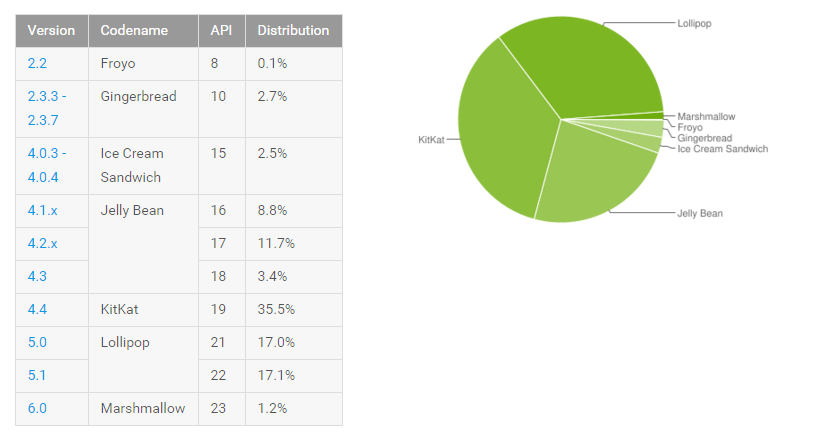
\includegraphics[width=1\textwidth]{figures/android_versionen.png}
	\captionof{figure}{Android Plattform Versionen \cite{platform:versions}}
	\label{figure:androidVersionen}
	\vspace{2ex}
\end{minipage}
 
Die Beispielimplementierung ist kompatibel mit der Android Version 5.0 und höher, da für das Anzeigen der Daten eine Funktionalität benötigt wird, die erst in der API Version 21 enthalten ist. Die App kann dadurch auf mehr als einem Drittel der vertriebenen Geräte ausgeführt werden. Wenn ältere Geräte Systemupdates erhalten, erhöht sich diese Anzahl entsprechend. 

	
	
